\chapter{Performance Evaluation}
Here should be an introduction of what we will test (the emulator and/or the protocol). 
\section{Evaluation Points}
Here should be a list of all requirement that is tested and criteria for passed not passed. 
Requirements: 
\begin{itemize}
\item Emulator
	\begin{enumerate}
	\item Amount of users %(CPU,RAM) 
		\begin{itemize}
		\item Support TBD active users and TBD users total
		\end{itemize}
	\item Configurable %(Channel, Number of UEs, etc.)
		\begin{itemize}
		\item Changeable parameters: Channel type, path loss, number of devices, data profile
		\end{itemize}
	\item Power control 
		\begin{itemize}
		\item Should support a output power up to 23 dB with a range of TBD dB
		\end{itemize}
	\end{enumerate}
\item Protocol
	\begin{enumerate}[resume]
	\item  Ultra-low Complexity Devices
		\begin{itemize}
		\item The \gls{UE} has a sample rate of 240 KHz
		\item Only supports \gls{TBCC}
		\item Half-duplex
		\item Uses \gls{SISO} connection
		\end{itemize}
	\item Improved Coverage
		\begin{itemize}
		\item Support a \gls{MCL} of 164 dB
		\item Improve coverage by introducing \gls{CE} levels 
		\end{itemize}
	\item Support Massive Number of Devices 
		\begin{itemize}
		\item Support 52547 devices per cell-site sector based on a TBD data profile
		\end{itemize}
	\item Improved Power Efficiency
		\begin{itemize}
		\item  Achieve a battery life time of 10 years with a battery capacity of 5 Wh
		\item Using \gls{CE} to minimize Power amplifier backoff increasing efficiency
		\item Utilize \gls{cDRX}, \gls{eDRX} and \gls{PSM} to increase efficiency
	\end{itemize}
	\item Deployment flexibility
		\begin{itemize}
		\item The system should be able to be deployed inside legacy \gls{LTE}.
		\item The system should be able to be deployed as a stand alone solution.
		\end{itemize}
	\end{enumerate}
\end{itemize}
%\item Massiveness
%	\begin{enumerate}
%	\item Time to connect vs. connection request per second 
%	\item Data rate vs. number of users
%	\item Spectrum use vs. number of users
%	\item Interference level vs. number of users
%	\end{enumerate}
%\item Power
%	\begin{enumerate}
%	\item Energy consumption for attach.
%	\item Energy consumption vs. data rate
%	\item Energy consumption vs. coverage level
%	\item Energy consumption vs. operation mode
%	\item Energy consumption vs. number of UEs
%	\item Energy consumption vs. UE state (Connected (cDRX), eDRX, PSM, Off)
%	\end{enumerate}
%\end{enumerate}


Based on both the focus explained in \autoref{ch:Introduction} as well as some issues with the emulator explained TBD. The only points that is actually tested are:

\begin{itemize}
\item Emulator
	\begin{enumerate}
%	\item Amount of users %(CPU,RAM) 
	\item Configurable %(Channel, Number of UEs, etc.)
%	\item Power control 
	\end{enumerate}
\item Protocol
	\begin{enumerate}[resume]
%	\item Ultra-low Complexity Devices
%	\item Improved Coverage
%	\item Support Massive Number of Devices 
	\item Improved Power Efficiency
%	\item Deployment flexibility
	\end{enumerate}
\end{itemize}

\section{General Test Setup}
Here should be a description of the general setup (including figure) used in all test and a list of baseline values for all parameters. Including physical setup, BSE, UEE.

\begin{figure}[H]
\centering
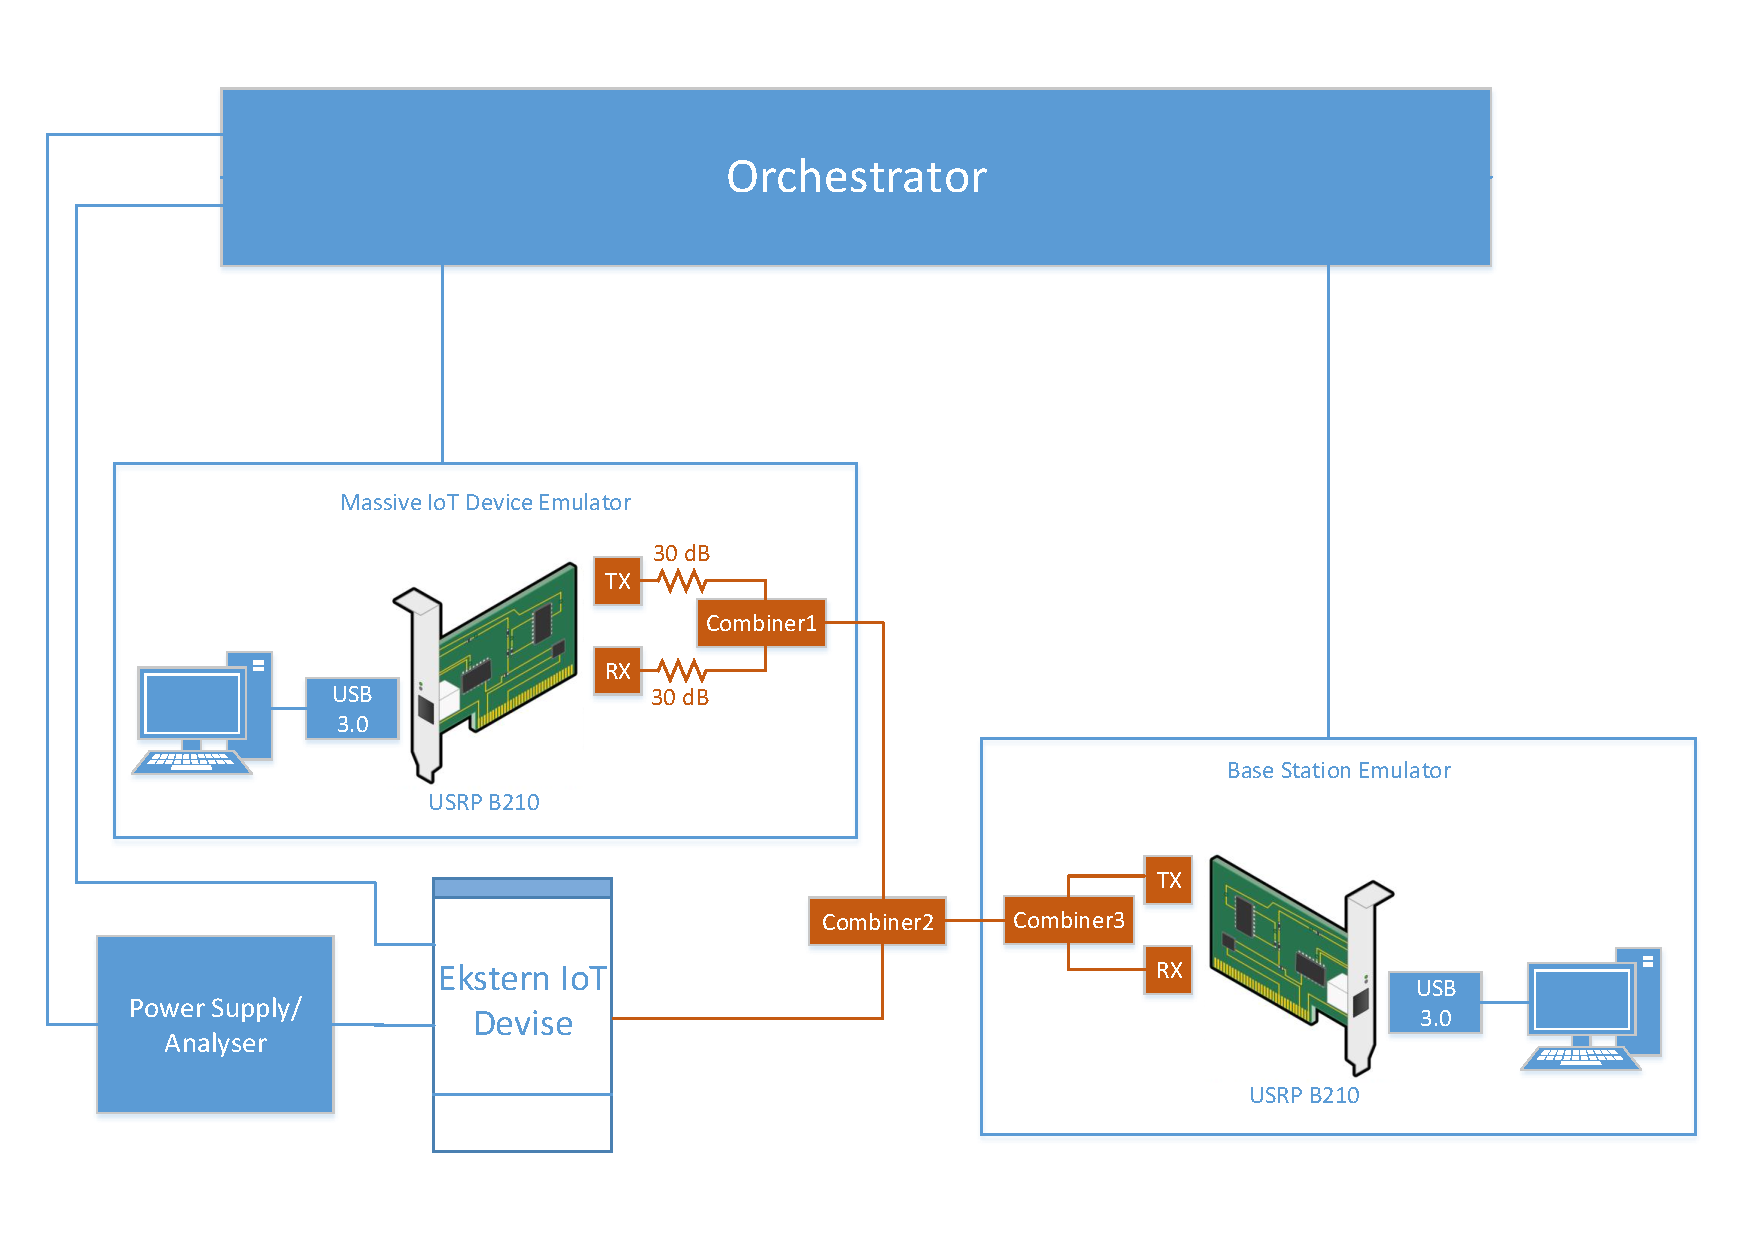
\includegraphics[width=\textwidth]{figures/General_test_setup.pdf}
\caption{General test setup}
\label{fig:General_test_setup}
\end{figure}

\begin{table}[H]
\centering
\resizebox{!}{0.5\textheight}{
\begin{tabular}{|l|l|}
\hline
\multicolumn{2}{|c|}{\textbf{Massive IoT Emulator}}                          \\ \hline
\textbf{Parameter} & \textbf{Value} \\ \hline
Number of devices  & 0              \\ \hline
Rx gain            & 40 dB          \\ \hline
Tx gain            & 40 dB          \\ \hline
R14                & False          \\ \hline
Dl\_EARFCN         & 6310           \\ \hline
UE\_category       & Nb1            \\ \hline
\multicolumn{2}{|c|}{\textbf{Power Supply/Analyser}}                         \\ \hline
Enable             & Off            \\ \hline
Volt               & 3.6 V          \\ \hline
Ampere             & 1 A            \\ \hline
\multicolumn{2}{|c|}{\textbf{Ekstern IoT device}}                            \\ \hline
Enable             & Off            \\ \hline
Dl\_EARFCN         & 6310           \\ \hline
\multicolumn{2}{|c|}{\textbf{Base Station Emulator}}                         \\ \hline
Cell type          & NB-IoT         \\ \hline
Number of cells    & 1              \\ \hline
Operation mode     & Standalone     \\ \hline
Dl\_EARFCN         & 6310           \\ \hline
Cell ID            & 0              \\ \hline
Tx gain            & 89 dB          \\ \hline
R14                & False          \\ \hline
nprach\_detect\_threshold  & 19 dB  \\ \hline
\end{tabular}
}
\caption{My caption}
\label{my-label}
\end{table}


\section{Evaluation}
%Here should be a step by step procedure of all test for all requirements, maybe put tapplans in appendix.

\subsection{Amount of Devices}

\subsection{Configurable}

\subsection{Power Control}

\subsection{Ultra-low Complexity Devices}

\subsection{Improved Coverage}

\subsection{Support Massive Number of Devices}

\subsection{Improved Power Efficiency}
\subsubsection{Test Overview}
\subsubsection{Test Setup}
\subsubsection{Test Procedure}
\subsection{Deployment Flexibility}

%\subsection{Battery Lifetime}
%From the model derived in \todo{make ref to bat model section} it can be found that the necessary parameters are:
%\begin{itemize}
%\item $P_device$
%\item 
%\end{itemize}

\section{Results}
Here should be a list of all results produced from the test. A short note should be attached to the results if the requirement is passed and if not why not.

\begin{table}[H]
\centering
\begin{tabular}{|l|l|} \hline
\textbf{Requirement}              & \textbf{Performance} \\ \hline
Amount of Devices                 &                      \\ \hline
Configurability                   &                      \\ \hline
Power Control                     &                      \\ \hline
Low Complexity Devices            &                      \\ \hline
Improved Coverage                 &                      \\ \hline
Support Massive Amount of Devices &                      \\ \hline
Improved Power Efficiency         &                      \\ \hline
Deployment Flexibility            &                      \\ \hline
\end{tabular}
\caption{My caption}
\label{my-label2}
\end{table}

%\section{Table Summary or Discussion}